\documentclass[12pt, a4paper, oneside]{ctexart}
\usepackage{amsmath, amsthm, amssymb, bm, color, graphicx, geometry, mathrsfs,extarrows, braket, booktabs, array, xcolor, fontspec, appendix, float, subfigure, wrapfig}
\usepackage[colorlinks,linkcolor=red,anchorcolor=blue,citecolor=blue,urlcolor=blue,menucolor=black]{hyperref}

%%%% 设置中文字体 %%%%
\setCJKmainfont{方正新书宋_GBK.ttf}[ BoldFont = 方正小标宋_GBK, ItalicFont = 方正楷体_GBK]
%%%% 设置英文字体 %%%%
\setmainfont{Times New Roman}
\setsansfont{Calibri}
\setmonofont{Consolas}

%%%% 设置代码块 %%%%
% 在vscode中使用minted需要先配置python解释器, Ctrl+Shift+P, 输入Python: Select Interpreter选择安装了Pygments的Python版本. 再在setting.json中xelatex和pdflatex的参数中加入 "--shell-escape", 即可
% TeXworks中配置方法参考: https://blog.csdn.net/RobertChenGuangzhi/article/details/108140093
\usepackage{minted}
\renewcommand{\theFancyVerbLine}{
    \sffamily\textcolor[rgb]{0.5,0.5,0.5}{\scriptsize\arabic{FancyVerbLine}}} % 修改代码前序号大小

\newmintinline{matlab}{fontsize=\small, linenos, breaklines, frame=lines}  % 使用\cppinline{代码}
\newminted{matlab}{fontsize=\small, mathescape, linenos, breaklines, frame=lines}  % 使用\begin{cppcode}代码\end{cppcode}
\newmintedfile{matlab}{fontsize=\small, linenos, breaklines, frame=lines}  % 使用\pythonfile{代码地址}
\newmintinline{python}{fontsize=\small, linenos, breaklines, frame=lines, python3}  % 使用\pythoninline{代码}
\newminted{python}{fontsize=\small, linenos, breaklines, frame=lines, python3}  % 使用\begin{pythoncode}代码\end{pythoncode}
\newmintedfile{python}{fontsize=\small, linenos, breaklines, frame=lines, python3}  % 使用\pythonfile{代码地址}

%%%% 设置行间距与页边距 %%%%
\linespread{1.2}
\geometry{left=2.5cm, right=2.5cm, top=2.5cm, bottom=2.5cm}

%%%% 定理类环境的定义 %%%%
\newtheorem{example}{例}            % 整体编号
\newtheorem{theorem}{定理}[section] % 定理按section编号
\newtheorem{definition}{定义}
\newtheorem{axiom}{公理}
\newtheorem{property}{性质}
\newtheorem{proposition}{命题}
\newtheorem{lemma}{引理}
\newtheorem{corollary}{推论}
\newtheorem{remark}{注解}
\newtheorem{condition}{条件}
\newtheorem{conclusion}{结论}
\newtheorem{assumption}{假设}
\numberwithin{equation}{section}  % 公式按section编号 (公式右端的小括号)
\newtheorem{algorithm}{算法}
\newsavebox{\nameinfo}
\renewenvironment{myTitle}[1]{
    \begin{center}
    {\zihao{-2}\bf #1\\}
    \zihao{-4}\it
}{\end{center}}  % \begin{myTitle}{标题内容}作者信息\end{myTitle}

%%%% 图片相对路径 %%%%
\graphicspath{{figure/}} % 当前目录下的figure文件夹, {../figure/}则是父目录的figure文件夹
\setlength{\abovecaptionskip}{-0.2cm}  % 缩紧图片标题与图片之间的距离
\setlength{\belowcaptionskip}{0pt} 

\everymath{\displaystyle} % 默认全部行间公式, 想要变回行内公式使用\textstyle
\DeclareMathOperator*\uplim{\overline{lim}}     % 定义上极限 \uplim_{}
\DeclareMathOperator*\lowlim{\underline{lim}}   % 定义下极限 \lowlim_{}
\DeclareMathOperator*{\argmax}{arg\,max}  % \argmin
\DeclareMathOperator*{\argmin}{arg\,min}  % \argmax
\let\leq=\leqslant % 简写小于等于\leq (将全部leq变为leqslant)
\let\geq=\geqslant % 简写大于等于\geq (将全部geq变为geqslant)

%%%% 一些宏定义 %%%%%
\def\bd{\boldsymbol}        % 加粗(向量) boldsymbol
\def\disp{\displaystyle}    % 使用行间公式 displaystyle(默认)
\def\tsty{\textstyle}       % 使用行内公式 textstyle
\def\sign{\text{sign}}      % sign function
\def\wtd{\widetilde}        % 宽波浪线 widetilde
\def\R{\mathbb{R}}          % Real number
\def\C{\mathbb{C}}          % Complex number
\def\Q{\mathbb{Q}}          % Rational number
\def\N{\mathbb{N}}          % Natural number
\def\Z{\mathbb{Z}}          % Integer number
\def\d{\mathrm{d}}          % differential operator
\def\e{\mathrm{e}}          % Euler's number
\def\i{\mathrm{i}}          % imaginary number
\def\re{\mathrm{Re}}        % Real part
\def\im{\mathrm{Im}}        % Imaginary part
\def\L{\mathcal{L}}         % Loss function
\def\wdh{\widehat}          % 宽帽子 widehat
\def\ol{\overline}          % 上横线 overline
\def\ul{\underline}         % 下横线 underline
\def\add{\vspace{1ex}}      % 增加行间距
\def\del{\vspace{-1.5ex}}   % 减少行间距

%%%% 正文开始 %%%%
\begin{document}
\begin{title}{CVPR第三次作业-相机标定}
    强基数学002\\
    吴天阳\quad 2204210460,马煜璇\quad 2204220461,陈博\quad 2203623001
\end{title}
% \setcounter{section}{1}
\section{实验目的}
1、掌握针孔相机成像的原理与特点;

2、掌握针孔成像系统中的坐标系(世界坐标、摄像机坐标、成像平面坐标、图像坐标)及各个坐标系之间关系;

3、掌握针孔相机模型中内参数与外参数的物理意义;掌握相机的经向畸变与切向畸变的特点及校正方法;

4、掌握基于平面模式的相机标定原理(张氏标定法);

5、统计分析标定误差形成原因,思考提升标定参数精度的方法。
\section{实验原理}
\subsection{针孔成像原理及特点}
\textbf{针孔成像原理}:将三维欧式空间中点$P(X,Y,Z),\ (Z\neq 0)$,通过中心$O$(相机镜头透镜)的射线与成像平面的交点$p$,称为$P$的中心投影像点. 其中成像平面是不过原点$O$的平面,我们假设成像平面为$z=1$,则通过向量等比例缩放可得投影像点为$p'(X/Z,Y/Z,1)$.

\textbf{针孔成像特点}:

1. 近大远小:假设三维空间中高为$h$的柱子,上端点位于$(X,Y+h, Z)$,下端点位于$(X,Y,Z)$,则成像结果分别为$(X/Z,(Y+h)/Z,1),\ (X/Z,Y/Z,1)$,则成像平面上两点高度差为$h'=h/Z$,若$Z$越大则$h'$越小,$Z$越小则$h'$越大,即近大远小.

2. 平行线汇聚一点:设$A,B,C$是三维空间中的三条向量,$\alpha_1,\ \alpha_2$分别从$A,B$出发沿着方向$C$传播,则$\alpha_1(\lambda):A+\lambda C$,$\alpha_2(\lambda):B+\lambda C$,则$\alpha_1,\alpha_2$在成像平面上的投影分别为
\begin{align*}
    \beta_1(\lambda) =&\ \left(\frac{A_x+\lambda C_x}{A_z+\lambda C_z},\frac{A_y+\lambda C_y}{A_z+\lambda C_z},1\right)\to \left(\frac{C_x}{C_z},\frac{C_y}{C_z},1\right),\ (\lambda \to \infty),\\
    \beta_1(\lambda) =&\ \left(\frac{B_x+\lambda C_x}{B_z+\lambda C_z},\frac{B_y+\lambda C_y}{B_z+\lambda C_z},1\right)\to \left(\frac{C_x}{C_z},\frac{C_y}{C_z},1\right),\ (\lambda \to \infty).
\end{align*}
这说明两条射线在相平面上投影的极限区域趋于一点,且起点分别为$\left(\frac{A_x}{A_z},\frac{A_y}{A_z},1\right)$和$\left(\frac{B_x}{B_z},\frac{B_y}{B_z},1\right)$,所以两条平行线投影到相平面上不再保持平行,称为\textbf{消失点}.\add

3. 无限延长平面汇聚成一条线:设三维平面为$N_xX+N_yY+N_zZ=  d$,其中$(N_x,N_y,N_z)$是三维平面的法向量,则投影到二维平面上为
\begin{equation*}
    N_xX/Z+N_yY/Z+N_z=N_xx+N_yy+N_z=d/Z\to 0,\quad (\lambda\to\infty)   
\end{equation*}
则其收敛到投影平面上的直线,称为\textbf{消失线}.
\subsection{针孔成像系统中的坐标系}
\begin{figure}[htbp]
    \centering
    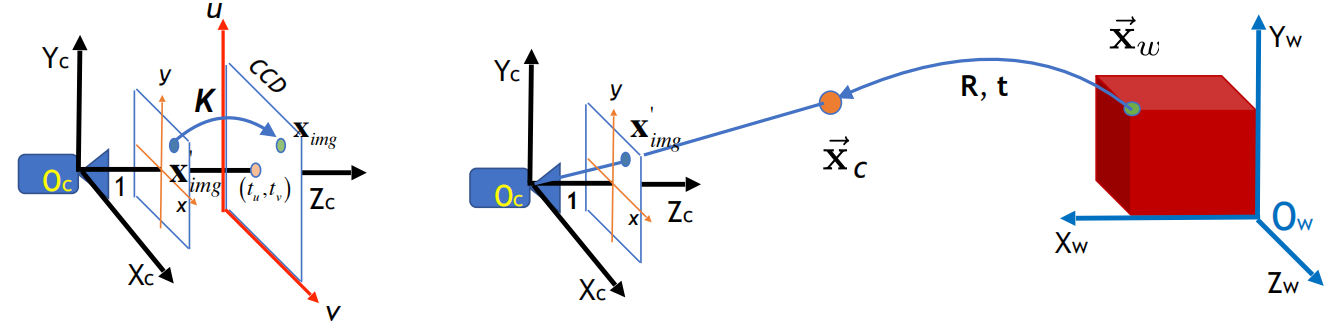
\includegraphics[scale=0.55]{坐标系转换.png}
    \caption{\label{fig-1}四种坐标系转换}
\end{figure}
1. 世界坐标系:三维空间中建立的基准坐标系,用于标记空间点和摄像机位置,如图\ref{fig-1}中坐标系$O_w\text{-}X_wY_wZ_w$所示.

2. 摄像机坐标系:以摄像机中心$O_c$作为原点,从$O_c$出发垂直于成像平面的射线作为主轴$Z_c$,从$O_c$出发与像平面水平平行作为$X_c$轴,从$O_c$出发与像平面平行且铅垂直作为$Y_c$轴,如图\ref{fig-1}中坐标系$O_c\text{-}X_cY_cZ_c$所示.

3. 成像平面坐标系(规范化坐标系):假设焦距为$f=1$,则成像平面为摄像机坐标系中$Z_c=1$的平面,记成像平面与$Z_c$的交点为原点$p$,以像平面水平线和铅垂线分别为$x$轴与$y$轴,如图\ref{fig-1}中坐标系$p\text{-}xy$所示.

4. 图像坐标系:原点$o$位于图像的左下角,平行于$x$轴作为$u$轴,平行于$y$轴作为$v$轴,如图\ref{fig-1}中坐标系$o\text{-}uv$所示.

这里需要引入\textbf{齐次坐标}概念,设三维坐标$\bd{x}(X,Y,Z)$,则其对应的齐次坐标为四维坐标$\bd{x'}(X,Y,Z,1)$,升维以后的齐次坐标能够通过矩阵完成平移操作,便于表示. 以下坐标定义均为齐次坐标.

我们记三维空间中物体的世界坐标为$\bd{x}_w$,摄像机坐标为$\bd{x}_c$(单位:m或mm),成像平面坐标为$\bd{x}'_{img}$,图像坐标为$\bd{x}_{img}$(单位:像素).

则四个坐标系的转换关系如下图所示
\begin{figure}[htbp]
    \centering
    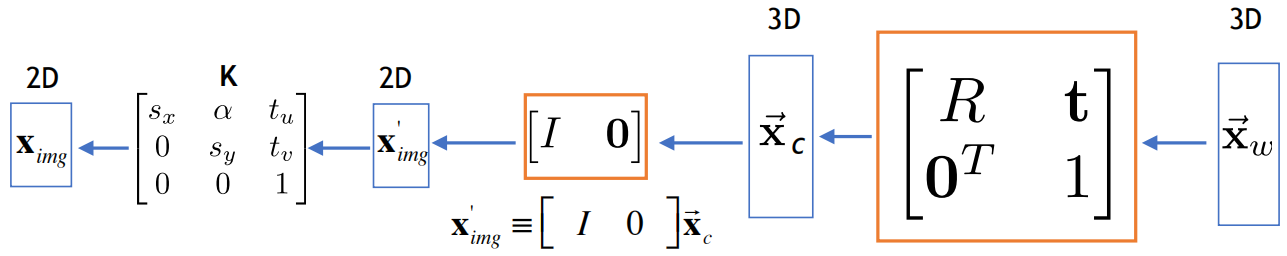
\includegraphics[scale=0.55]{转换坐标.png}
    \caption{\label{fig-2}四种坐标转换矩阵}
\end{figure}

上图变换主要包含三个矩阵:

1. 外参矩阵:$4\times 4$矩阵,包括$3\times 3$的旋转矩阵$R$以及一个$3\times 1$的平移向量$\bd{t}$. 该矩阵会随着物体或相机的移动而发生变化.

2. 投影矩阵:$3\times 4$矩阵,取前三维分量,然后转化为齐次坐标,转化符号记为$\equiv$. 注意,该过程会产生尺度因子$\lambda$,即缩放比例. 如下式所示
\begin{equation*}
    [I\quad 0]\bd{x}_c = \left[\begin{matrix}
        1&0&0&0\\0&1&0&0\\0&0&1&0
    \end{matrix}\right]
    \left[\begin{matrix}
        X_c\\Y_c\\Z_c\\1
    \end{matrix}\right]=\left[\begin{matrix}
        X_c&Y_c&Z_c
    \end{matrix}\right]\equiv\left[\begin{matrix}
        X_c/Z_c\\Y_c/Z_c\\1
    \end{matrix}\right] = \bd{x}'_{img}
\end{equation*}
其中$[I\quad 0]\bd{x}_c = \lambda \bd{x}'_{img}$,$\lambda = 1/Z_c$.

3. 内参矩阵$K$:$3\times 3$矩阵,将像素从成像坐标系转化到图像坐标系中,由相机的自有特性决定,不随外部物体变化而变化. 其具体表示如下
\begin{equation*}
    K = \left[\begin{matrix}
        f_x&\alpha&t_u\\
        0&f_y&t_v\\
        0&0&1
    \end{matrix}\right]
\end{equation*}
其中$(t_u,t_v)$表示图像坐标系原点在成像坐标系中所处的位置. 由于需要从单位m或mm转化为像素,所以还需要$f_x,\ f_y$分别表示沿$x$与$y$轴的缩放比例(相机焦距),由于$o\text{-}uv$不一定正交,所以还存在倾斜因子$\alpha$.

\subsection{相机径向畸变与切向畸变的特点及矫正方法}
在实际应用中,由于光学透镜不是完美的,通过透镜边缘的光线会发生偏转,导致偏离成像位置,发生扭曲,称为光学畸变. 光学畸变主要分为两种:

1. 径向畸变:主要由透镜问题产生,是一种非线性扭曲,畸变程度取决于与主点的距离,光线距离透镜中心越远,畸变效果更为严重. 有枕形畸变和桶形畸变两种.
\begin{figure}[htbp]
    \centering
    \subfigure[桶形畸变]
    {
        \begin{minipage}[b]{0.45\linewidth}
            \centering
            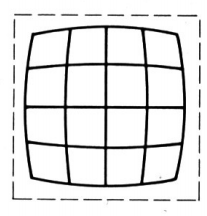
\includegraphics[scale=0.8]{桶形畸变.png}
        \end{minipage}
    }
    \subfigure[枕形畸变]
    {
        \begin{minipage}[b]{0.45\linewidth}
            \centering
            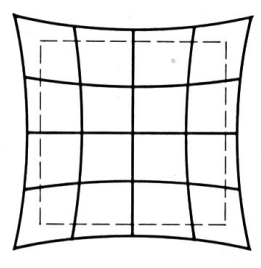
\includegraphics[scale=0.6]{枕形畸变.png}
        \end{minipage}
    }
\end{figure}

2. 在摄像机安装过程中,光轴与成像平面无法完成平行,导致切向畸变.

两种畸变可用如下模型表示:
\begin{equation*}
    \hspace*{-2cm}
    \begin{cases}
        x_d-x_c=\overbrace{(x_u-x_c)(1+k_1r^2+k_2r^4+\cdots)}^{\text{径向畸变}}+\overbrace{\left[p_1(r^2+2(x_u-x_c)^2)+2p_2(x_u-x_c)(y_u-y_c)\right](1+p_3r^2+\cdots)}^{\text{切向畸变}}\\
        y_d-y_c=(y_u-y_c)(1+k_1r^2+k_2r^4+\cdots)+\left[p_2(r^2+2(y_u-y_c)^2)+2p_1(x_u-x_c)(y_u-y_c)\right](1+p_3r^2+\cdots)\\
    \end{cases}
\end{equation*}
(下述坐标均在成像坐标系中)其中$(x_u,y_u)$表示理想像素点坐标,$(x_d,y_d)$表示畸变图像点坐标,$(x_c,y_c)$表示畸变中心,$k_n$为镜像畸变系数,$p_n$为切向畸变系数,$r^2=(x_u-x_c)^2+(y_u-y_c)^2$.

令$(x_c,y_c)=(0,0)$,略去部分高阶项,可得简化版畸变模型
\begin{equation}
    \label{eq-简化畸变模型}
    \begin{cases}
        x_d=x_u(1+k_1r^2+k_2r^4)+p_1(r^2+2x_u^2)+2p_2x_uy_u\\
        y_d=y_u(1+k_1r^2+k_2r^4)+p_2(r^2+2y_u^2)+2p_1x_uy_u\\
    \end{cases}
\end{equation}
通过对畸变参数$k_1,k_2,p_1,p_2$进行求解后,反解求得理想像素点坐标$(x_u,y_u)$.
\subsection{张氏标定法}
由于世界坐标系可以自由设定,我们不妨取三维平面中的黑白棋盘作为$xOy$平面,则棋盘上的点均有$Z_w = 0$,由相机成像原理可知
\begin{equation*}
    x_{img} = \left[\begin{matrix}
        u\\v\\1
    \end{matrix}\right]\equiv K[R\quad \bd{t}]x_w = K[\bd{r}_1\quad \bd{r}_2\quad \bd{r}_3\quad \bd{t}]\left[\begin{matrix}
        X_w\\Y_w\\0\\1
    \end{matrix}\right] = K[\bd{r}_1\quad \bd{r}_2\quad \bd{t}]\left[\begin{matrix}
        X_w\\Y_w\\1
    \end{matrix}\right] = H\left[\begin{matrix}
        X_w\\Y_w\\1
    \end{matrix}\right]
\end{equation*}
其中$H$矩阵称为棋盘平面与图像平面之间的\textbf{单应性}(Homography)变换矩阵,由于尺度因子的省略,$H$矩阵对应了相机平面到\textbf{全体同一偏转角度棋盘平面}的一个同态映射.

通过大量的像素坐标以及对应的棋盘格坐标,可建立多个关于$H$的方程组,$H$为$3\times 3$矩阵,但由于存在一个尺度因子,所以共有$8$个待定参数. 一组对应坐标可以得到两个方程,所以至少$4$组对应坐标,更多的对应坐标可以通过最小二乘法估计得到$H$矩阵. 下面通过$H$矩阵分别求解内参矩阵$K$,外参矩阵以及径向畸变估计.

\subsubsection{估计相机内参矩阵}\del
\begin{equation}
    \label{eq-1}
    H = [\bd{h}_1\quad \bd{h}_2\quad \bd{h}_3] = \lambda K[\bd{r}_1\quad \bd{r}_2\quad \bd{t}]\Rightarrow\begin{cases}
        \bd{r}_1 = \frac{1}{\lambda}K^{-1}\bd{h}_1,\add\\
        \bd{r}_2 = \frac{1}{\lambda}K^{-1}\bd{h}_2.
    \end{cases}
\end{equation}
由于$\bd{r}_1\perp \bd{r}_2,\ ||\bd{r}_1||=||\bd{r}_2||$,于是
\begin{equation}
    \label{eq-2}
    \begin{cases}
        \bd{h}_1^T(K^{-1})^TK^{-1}\bd{h}_2 = 0,\\
        \bd{h}_1^T(K^{-1})^TK^{-1}\bd{h}_1 = \bd{h}_2^T(K^{-1})^TK^{-1}\bd{h}_2,\\
    \end{cases}
\end{equation}
令
\begin{equation*}
    B = (K^{-1})^TK^{-1} = \left[\begin{matrix}
        B_{11}&B_{12}&B_{13}\\
        B_{12}&B_{22}&B_{23}\\
        B_{13}&B_{23}&B_{33}\\
    \end{matrix}\right]
\end{equation*}
由于$B$矩阵是对称阵,所以只需确定下三角部分$6$个参数,令
\begin{equation*}
    \bd{b} = [B_{11}\quad B_{12}\quad B_{22}\quad B_{13}\quad B_{23}\quad B_{33}]^T
\end{equation*}
则上述方程\ref{eq-2}可表示为方程$\begin{cases}
    \bd{v}_{12}^T\bd{b} = 0,\\
    [\bd{v}_{11}^T-\bd{v}_{22}^T]\bd{b} = 0.
\end{cases}$,其中$\bd{v}_{ij}$由$H$矩阵确定,具体形式请见\url{https://zhuanlan.zhihu.com/p/136827980}. 由于每种不同角度的棋盘图像可以确定不同的$H$矩阵,从而确定$\bd{v}_{ij}$,于是每张不同角度的棋盘图像可以确定两个关于$\bd{b}$的方程,总共有$6$个待定参数,所以需要至少$3$张不同角度的棋盘才能唯一确定内参矩阵.

\subsubsection{估计相机外参矩阵}
有了内参矩阵$K$以后,我们通过式\ref{eq-1}可知
\begin{equation*}
    \lambda[\bd{r}_1\quad \bd{r}_2\quad \bd{t}] = K^{-1}[\bd{h}_1\quad \bd{h}_2\quad \bd{h}_3]
\end{equation*}
则
\begin{equation*}
    \begin{cases}
        \lambda = ||K^{-1}\bd{h}_1||_2 = ||K^{-1}\bd{h}_2||_2,\\
        \bd{t} = K^{-1}\bd{h}_3/\lambda,\\
        \bd{r}_1 = K^{-1}\bd{h}_1/\lambda,\\
        \bd{r}_2 = K^{-1}\bd{h}_2/\lambda,\\
        \bd{r}_3=\bd{r}_1\times \bd{r}_2.
    \end{cases}
\end{equation*}
其中$||\cdot||_2$为2-范数(欧式范数),于是外参矩阵为$[R\quad \bd{t}] = [\bd{r}_1\quad \bd{r}_2\quad \bd{r}_3\quad \bd{t}]$.

在实际应用中,由于数据中存在噪音,$R$矩阵不一定完全满足旋转矩阵的性质,所以通常使用奇异值分解求解$R$.

\subsubsection{最大似然估计}
在实际标定过程中,一般存在大量标定图片同时对参数进行估计,这时使用最大似然估计对上述算法进行优化. 假设有$n$张标定图片,每张图片中都有$m$个棋盘格角点,且棋盘格大小一致,棋盘中角点相对位置相同. 利用平方损失函数,构造最小化风险函数如下
\begin{equation*}
    \min_{K,\bd{k},R,\bd{t},\lambda}\frac{1}{n}\sum_{i=1}^n\sum_{j=1}^m\left|\left|x_{ij}-x'(K,\bd{k},R_i,\bd{t}_i,\lambda_i,X_{j})\right|\right|^2
\end{equation*}
其中$K$为内参矩阵,$\bd{k}$为径向畸变参数,$[R_i\quad \bd{t}_i]$为第$i$张图像对应的外参矩阵,$\lambda_i$为第$i$张图像对应的尺度因子,第$i$张图像中与棋盘中第$j$个角点坐标$X_{j}$对应的图像坐标为$x_{ij}$,$x'(\cdot)$为根据棋盘中角点坐标$X_{j}$以及由该图片对应的外参数矩阵$[R_i\quad \bd{t}_i]$、尺度因子$\lambda_i$及内参矩阵和径向畸变,预测得到的图像像素坐标.

\section{实验步骤与结果分析}
利用MATLAB工具箱Camera Calibration Toolbox for Matlab进行相机标定.
\subsection{提取棋盘格角点}
提取calib\_example中奇数编号的棋盘图片角点,角点矩阵大小为$12\times 13 = 156$,编号为3,5,7,9的图像角点检测结果如下图所示:
\begin{figure}[htbp]
    \centering
    \hspace*{-4cm}
    \subfigure
    {
        \begin{minipage}[b]{0.6\linewidth}
            \centering
            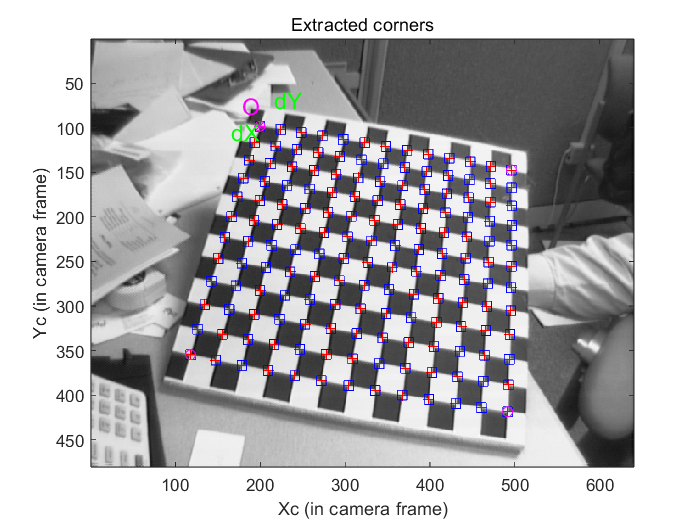
\includegraphics[scale=0.6]{角点1.png}
        \end{minipage}
        \begin{minipage}[b]{0.45\linewidth}
            \centering
            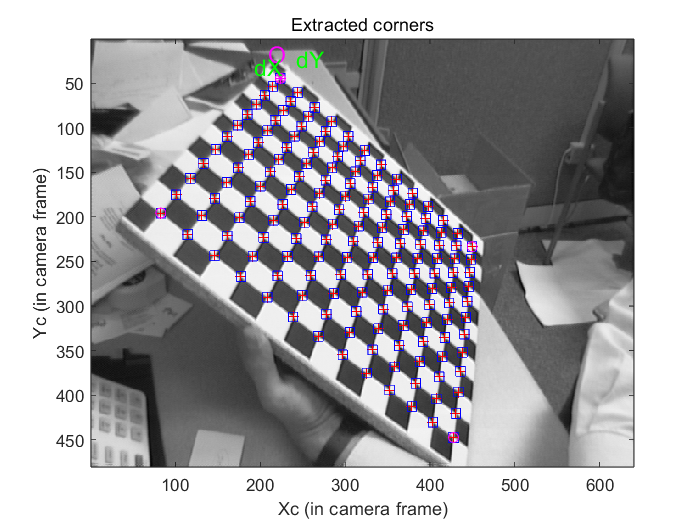
\includegraphics[scale=0.6]{角点2.png}
        \end{minipage}
    }
    \hspace*{-4cm}
    \subfigure
    {
        \begin{minipage}[b]{0.6\linewidth}
            \centering
            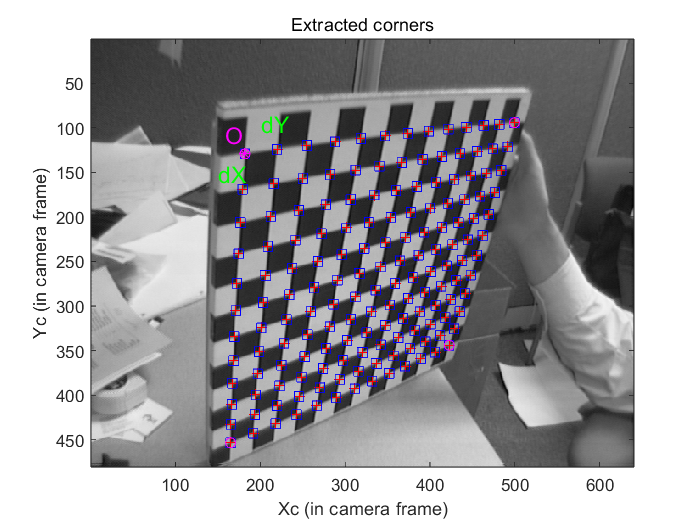
\includegraphics[scale=0.6]{角点3.png}
        \end{minipage}
        \begin{minipage}[b]{0.45\linewidth}
            \centering
            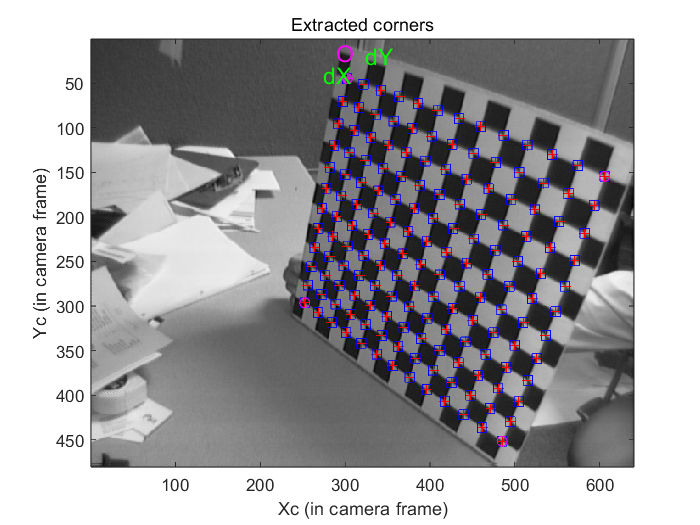
\includegraphics[scale=0.6]{角点4.png}
        \end{minipage}
    }
\end{figure}
\subsection{求解单应性矩阵}
通过compute\_homography.m文件计算每幅图像的单应性矩阵,下面通过上述角点检测计算出的$x,X$数组,分别为图像坐标和世界坐标,要求大小为$3\times 156$,但$x$矩阵为$2\times 156$,所以需要增加全为$1$的一行,$X$矩阵为$3\times 156$,但最下一行为$0$,所以需要做前两行的切片,再增加全为$1$的一行位于最下. 代码如下
\begin{matlabcode}
function [H] = calc_homography(x, X)
    shape = size(x);
    x_camera = [x; ones(1, shape(2))];
    x_world = [X(1:2,:); ones(1, shape(2))];
    H = compute_homography(x_camera, x_world);
end
\end{matlabcode}
得到图像奇数图像的$H$矩阵如下所示
\matlabfile{H_matrix.txt}
通过逆变换,加深理解. 这里以图像1,3的逆变换为例,其逆矩阵如下所示:
\matlabfile{invH_matrix.txt}
逆变换效果,得到棋盘平面的正投影,利用第二次作业双线性插值完成像素获取,代码及效果如下图所示:
\clearpage
\begin{figure}[htbp]
    \subfigure{
        \hspace*{-1.5cm}
        \begin{minipage}[b]{0.9\linewidth}
            \centering
            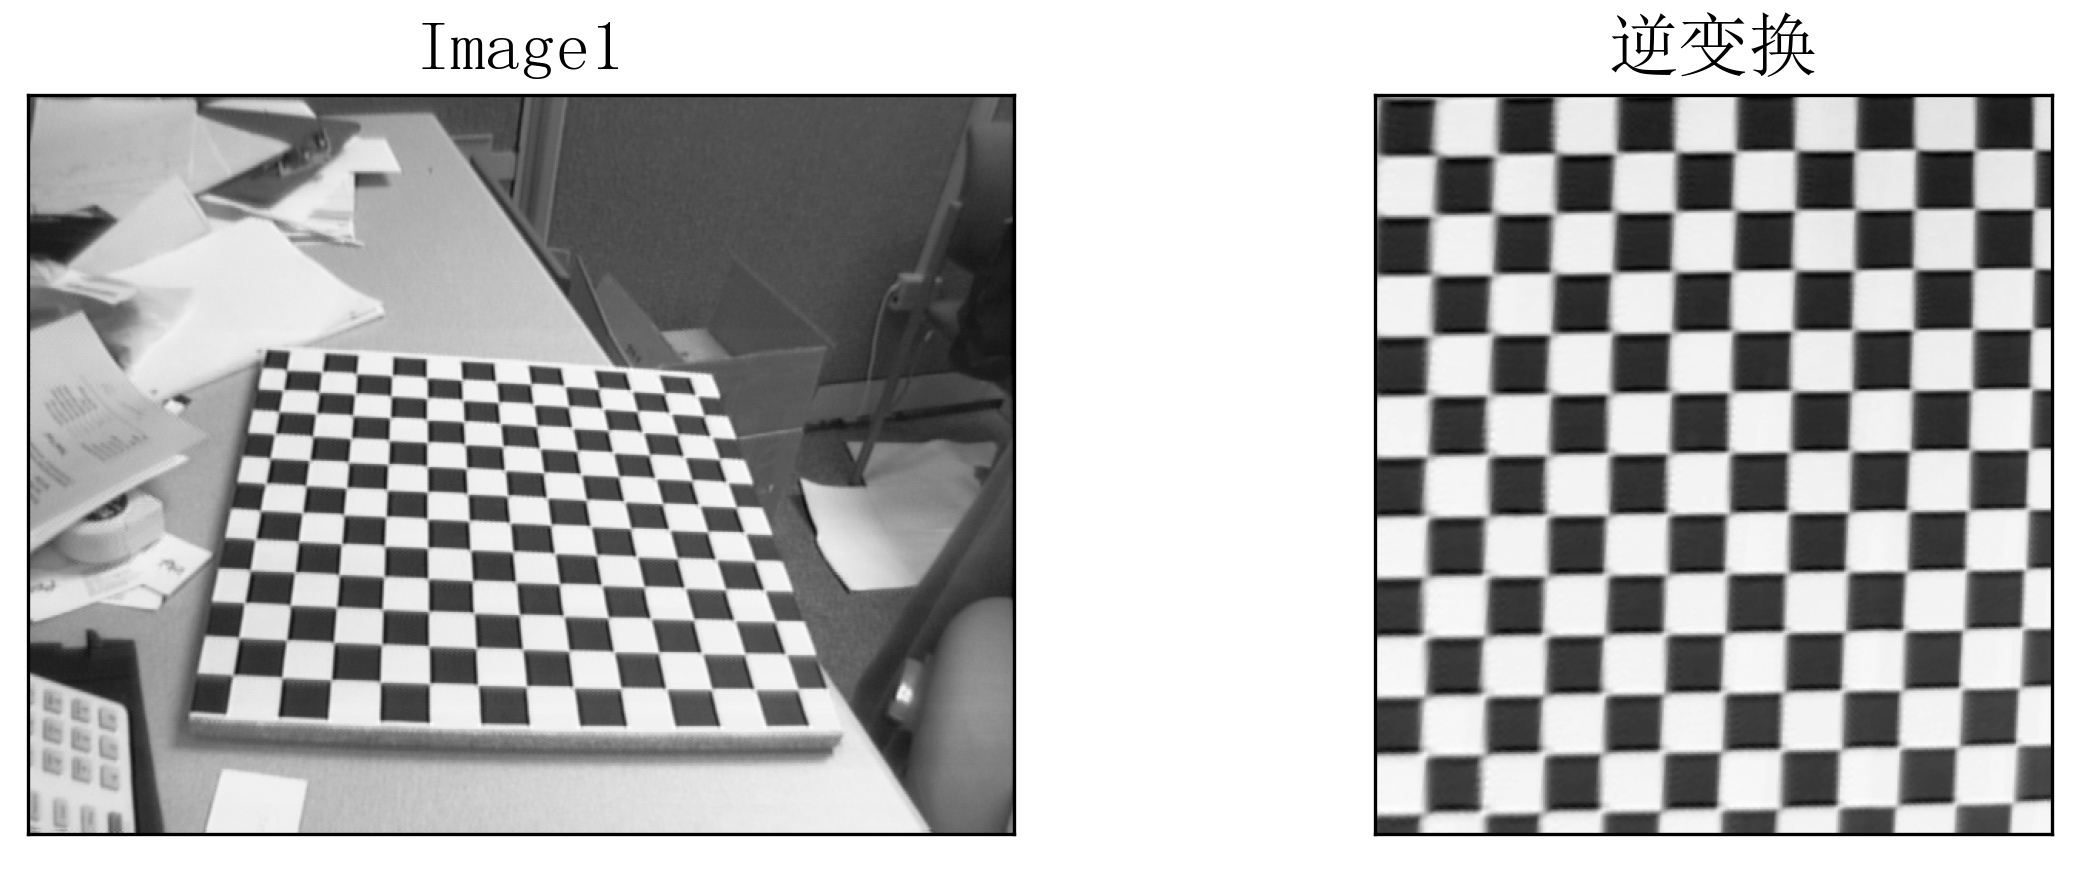
\includegraphics[scale=0.2]{Img1逆变换.png}
        \end{minipage}
    }
    \subfigure{
        \hspace*{-1.5cm}
        \begin{minipage}[b]{0.9\linewidth}
            \centering
            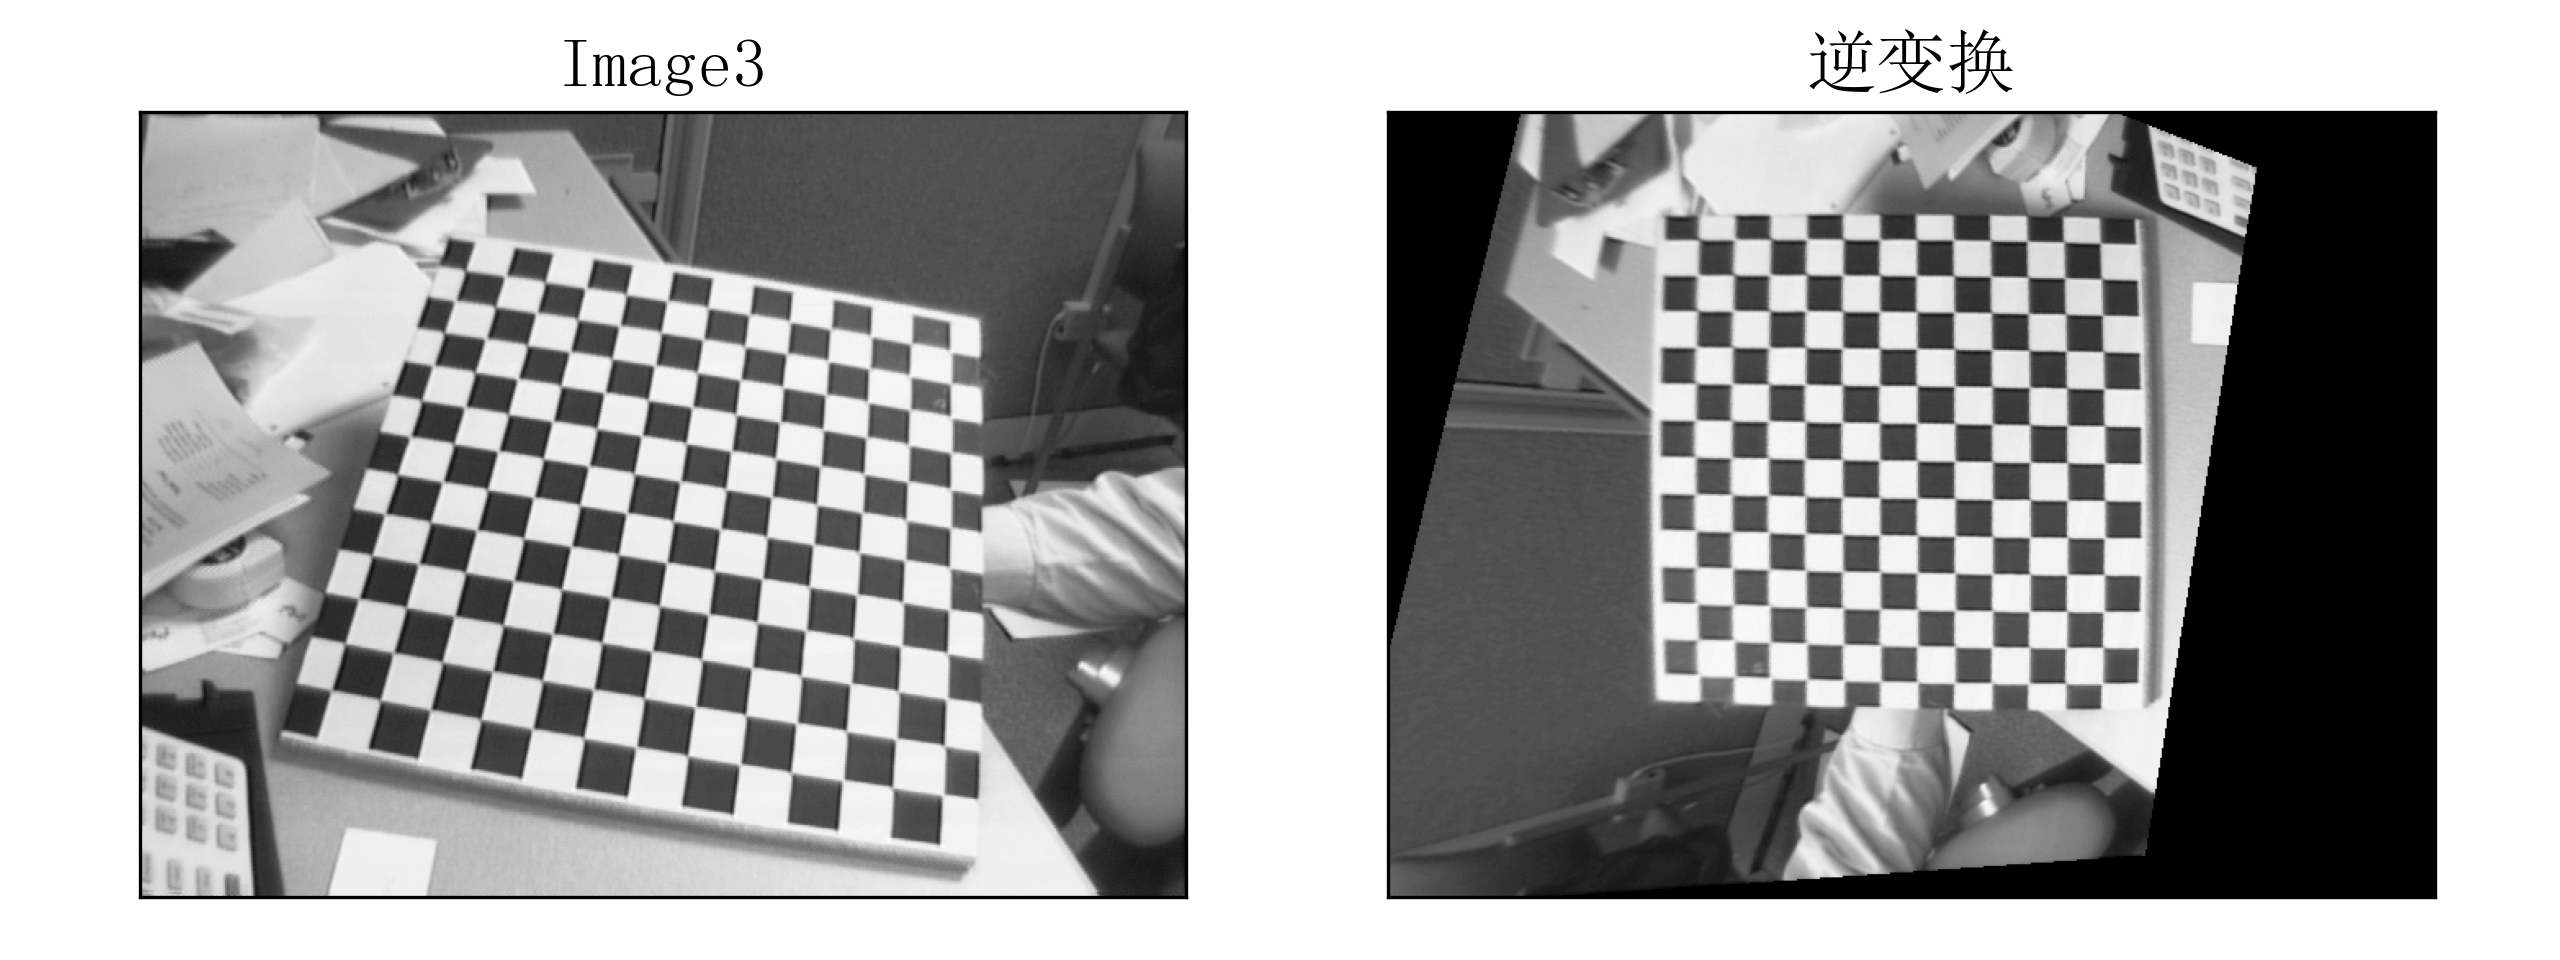
\includegraphics[scale=0.2]{Img3逆变换.png}
        \end{minipage}
    }
\end{figure}
\begin{pythoncode}
def transform(img, H):
H = H.T
n, m, c = img.shape
mid = np.array([n/2, m/2, 0])
H[2, :] += mid @ H - mid  # 中心化
output = np.zeros(img.shape)
for i in tqdm(range(n)):
    for j in range(m):
        x, y, z = (np.array([j, i, 1]) @ H)
        x /= z  # 正则化
        y /= z
        output[i, j, :] = bilinear_interpolate(img, y, x)  # 利用双线性插值
return output
\end{pythoncode}

\subsection{估计相机内参与外参}
\subsubsection{初始化内参}
利用init\_intrinsic\_param.m计算初始化内参矩阵,得到以下输出结果:
\matlabfile{内参.txt}
于是内参矩阵为
\begin{equation*}
    K = \left[\begin{matrix}
        668&0&319.5\\
        0&668&239.5\\
        0&0&1
    \end{matrix}\right]
\end{equation*}
由上述推导可知,约束条件为$\bd{r}_1\perp \bd{r}_2,\ ||\bd{r}_1|| = ||\bd{r}_2||$.

由于没有相机规格书,无法得知其物理含义.
\subsubsection{计算外参}
利用compute\_extrinsic\_init计算外参矩阵,返回值中的Tckk为平移向量,Rckk为旋转矩阵:
\begin{matlabcode}
function [out] = calc_external_par(x, X, fc, cc)
    [omckk,Tckk,Rckk] = compute_extrinsic_init(x,X,fc,cc,0,0);
    out = [[Rckk, Tckk]; zeros(1, 4)];
    out(4, 4) = 1;
end
\end{matlabcode}
于是外参矩阵为:
\matlabfile{外参.txt}
优化参数部分不理解原理无法实现.
\subsection{分析标定误差}
通过Calibration功能得到标定结果及误差(全部奇数张图片,共10张图片):
\begin{matlabcode}
Focal Length: fc = [ 661.07479   665.06267 ] +/- [ 1.91695   2.10219 ]
Principal point: cc = [ 303.25670   241.93662 ] +/- [ 3.53331   3.43451 ]
Skew: alpha_c = [ 0.00000 ] +/- [ 0.00000  ]   => angle of pixel axes = 90.00000 +/- 0.00000 degrees
Distortion: kc = [ -0.29392   0.38862   0.00060   -0.00101  0.00000 ] +/- [ 0.01548   0.06653   0.00084   0.00087  0.00000 ]
Pixel error: err = [ 0.57177   0.33143 ]
\end{matlabcode}
误差分布
\begin{figure}[htbp]
    \centering
    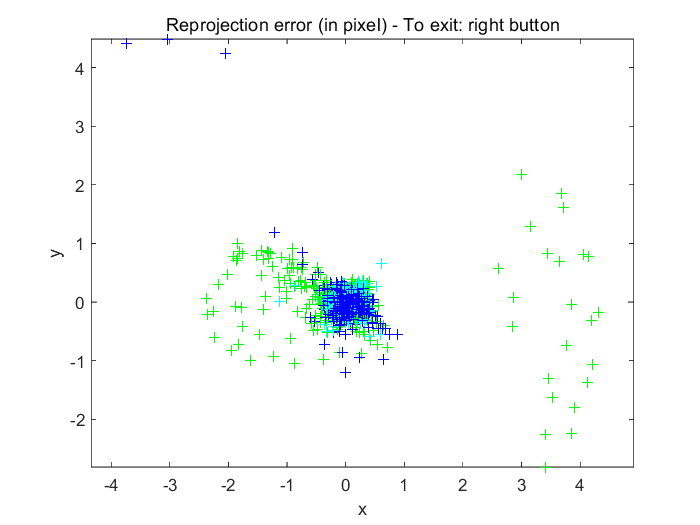
\includegraphics[scale=0.5]{error.png}
\end{figure}

通过Calibration功能得到标定结果及误差(全部奇数张图片,共5张图片):
\begin{matlabcode}
Focal Length: fc = [ 658.13644   658.74730 ] +/- [ 0.75708   0.81297 ]
Principal point: cc = [ 301.46396   246.52052 ] +/- [ 1.60017   1.55244 ]
Skew: alpha_c = [ 0.00000 ] +/- [ 0.00000  ]   => angle of pixel axes = 90.00000 +/- 0.00000 degrees
Distortion: kc = [ -0.26042   0.16194   0.00028   -0.00042  0.00000 ] +/- [ 0.00631   0.03001   0.00033   0.00036  0.00000 ]
Pixel error: err = [ 0.12323   0.11696 ]
\end{matlabcode}
误差分布
\begin{figure}[htbp]
    \centering
    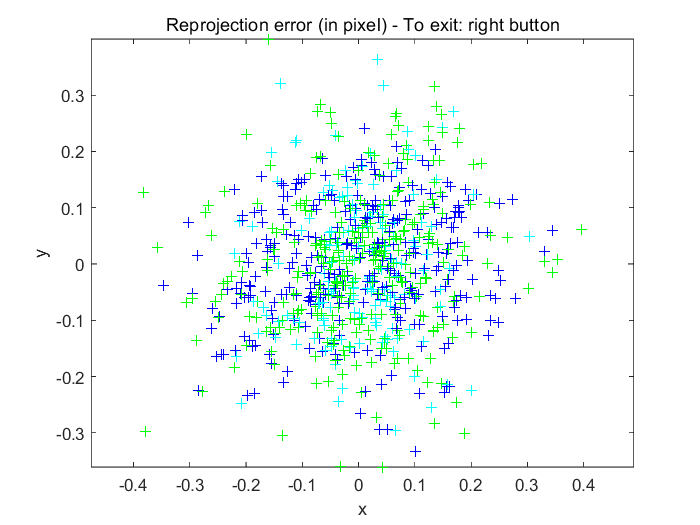
\includegraphics[scale=0.5]{error1.png}
\end{figure}

可以发现,虽然图像使用更多,但是可能导致噪声增多,误差分布中会出现较多的离散点,使得估计误差增大,而使用少量图像进行标定噪声数目较少,不会出现这种现象,说明每张标定图片降噪十分重要. 同时误差可能来源于由相机晶状体引起的图像畸变.


\section{结论与讨论}
通过本次实验,基本理解相机成像原理,以及张氏标定法具体计算方法. 利用MATLAB工具箱进行相机标定,通过角点检测,将图像坐标与三维网格坐标对应求解单应性矩阵,进而求解相机内参与外参,但由于没有具体相机参数,无法得知其物理含义. 在标定误差分析中,主要通过逆变换重构三维坐标得到误差大小. 对参数优化部分和具体误差分析部分仍有待进一步理解.

\end{document}

\iffalse
%%%% 表格模板 %%%%
\renewcommand\arraystretch{0.8} % 设置表格高度为原来的0.8倍
\begin{table}[!htbp] % table标准
    \centering % 表格居中
    \begin{tabular}{p{1cm}<{\centering}p{1cm}<{\centering}p{3cm}<{\centering}p{5cm}<{\centering}} % 设置表格宽度
    %\begin{tabular}{cccc}
        \toprule
        $x_i$ & $f[x_1]$ & $f[x_i, x_{i+1}]$ & $f[x_i, x_{i+1}, x_{i+2}]$ \\
        \midrule
        $x_0$ & $f(x_0)$ &                  &                          \\
        $x_0$ & $f(x_0)$ & $f'(x_0)$        &                          \\
        $x_0$ & $f(x_1)$ & $\frac{f(x_1)-f(x_0)}{x_1-x_0}$ & $\frac{f(x_1)-f(x_0)}{(x_1-x_0)^2}-\frac{f'(x_0)}{x_1-x_0}$\\
        \bottomrule
    \end{tabular}
\end{table}

%%%% 文字环绕图片, 标题加注释 %%%%
{ % 一般将文字环绕部分的图和文字, 用大括号括起来, 避免对文字外的格式发生影响
\begin{wrapfigure}[13]{r}{.5\linewidth} % 文字环绕行数为13行, 图片靠右 (l为靠左), 图片占0.5的行宽
    \centering
    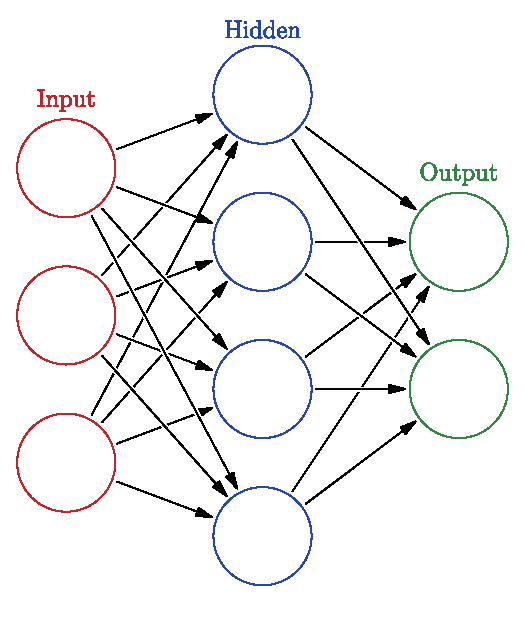
\includegraphics[scale=0.7]{neural_network.eps} % scale=0.7按比例缩放70%
    \caption{神经网络结构\protect\footnotemark[1]} % 记得加\protect, 设置1号脚标
    \label{figure-神经网络结构}
\end{wrapfigure}
\footnotetext[1]{图片来源: \url{https://en.wikipedia.org/wiki/File:Colored_neural_network.svg}}
文字文字
}

%%%% 普通图片, 标题加注释 %%%%
\begin{figure}[htbp] % h: 当前位置, t: 顶部, b: 底部, p: 浮动页, 这样组合指的是使用这个顺序进行排版
    \centering
    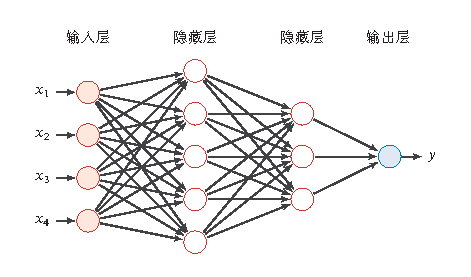
\includegraphics[scale=0.5]{前馈神经网络.eps}
    \caption{前馈神经网络\protect\footnotemark[1]}
    \label{figue-前馈神经网络}
\end{figure}
\footnotetext[1]{图片来源: 邱锡鹏, 神经网络与深度学习 \cite{ref-qxp}, 第92页}

%%%% 多组图 %%%%
    \begin{figure}[htbp]
        \centering
        \subfigure[迭代1次]  % 子图的标题
        {
            % 如果一行放三个图改成0.3\linewidth即可
            \begin{minipage}[b]{.45\linewidth}  % 0.45排版行距, 即一行放2个图, 一行放不下就换行
                \centering
                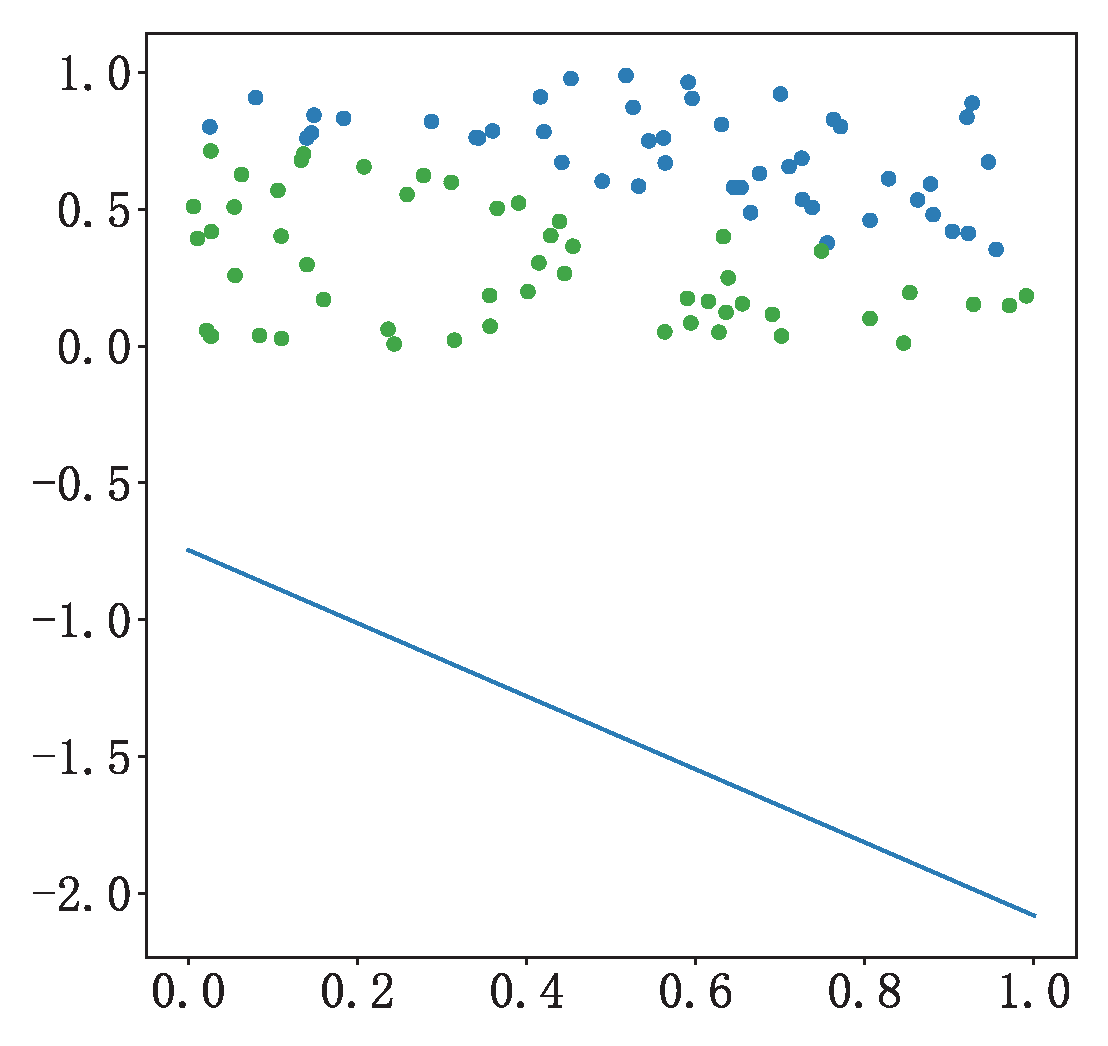
\includegraphics[scale=0.35]{1.eps}
            \end{minipage}
        }
        \subfigure[迭代100次]
        {
            \begin{minipage}[b]{.45\linewidth}
                \centering
                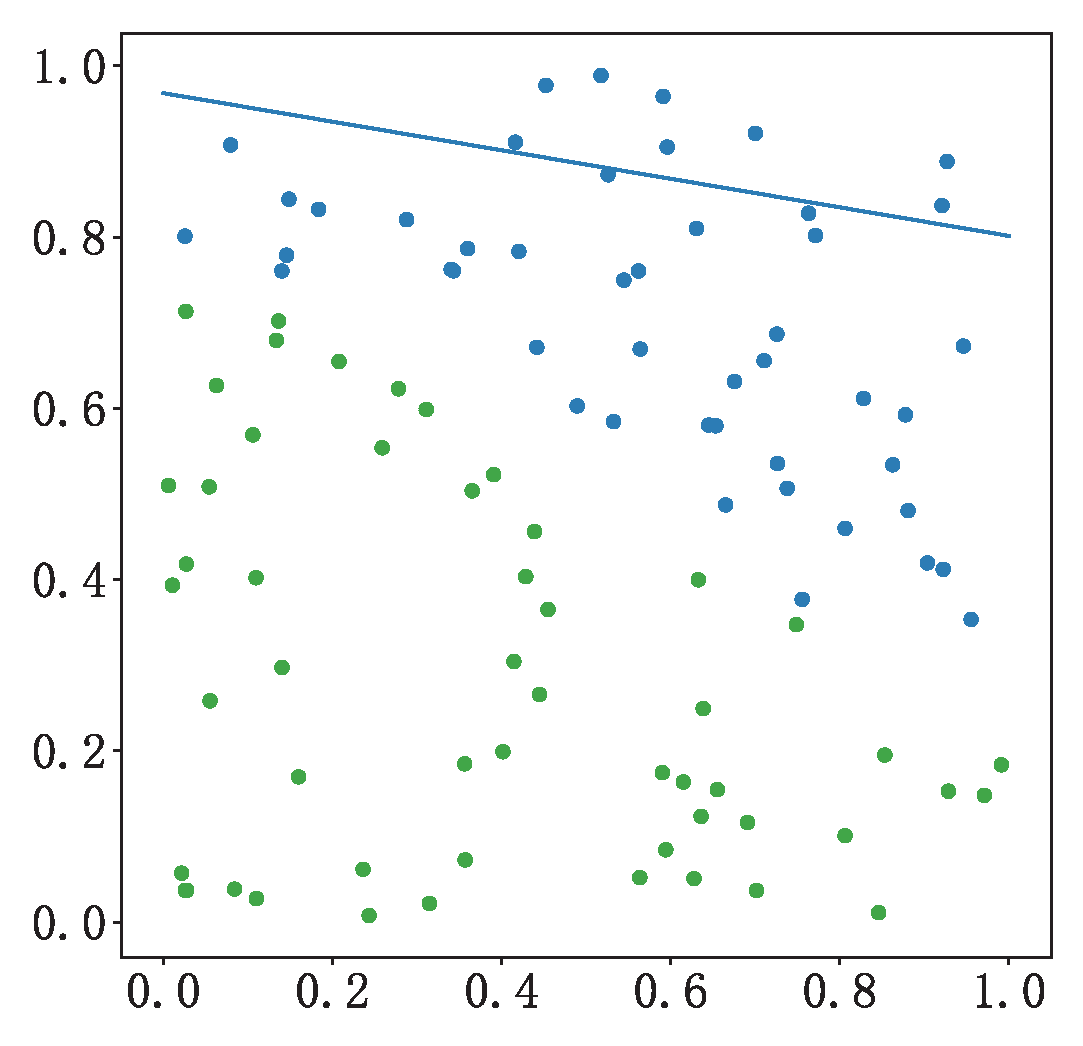
\includegraphics[scale=0.35]{100.eps}
            \end{minipage}
        }
        \subfigure[迭代500次]
        {
            \begin{minipage}[b]{.45\linewidth}
                \centering
                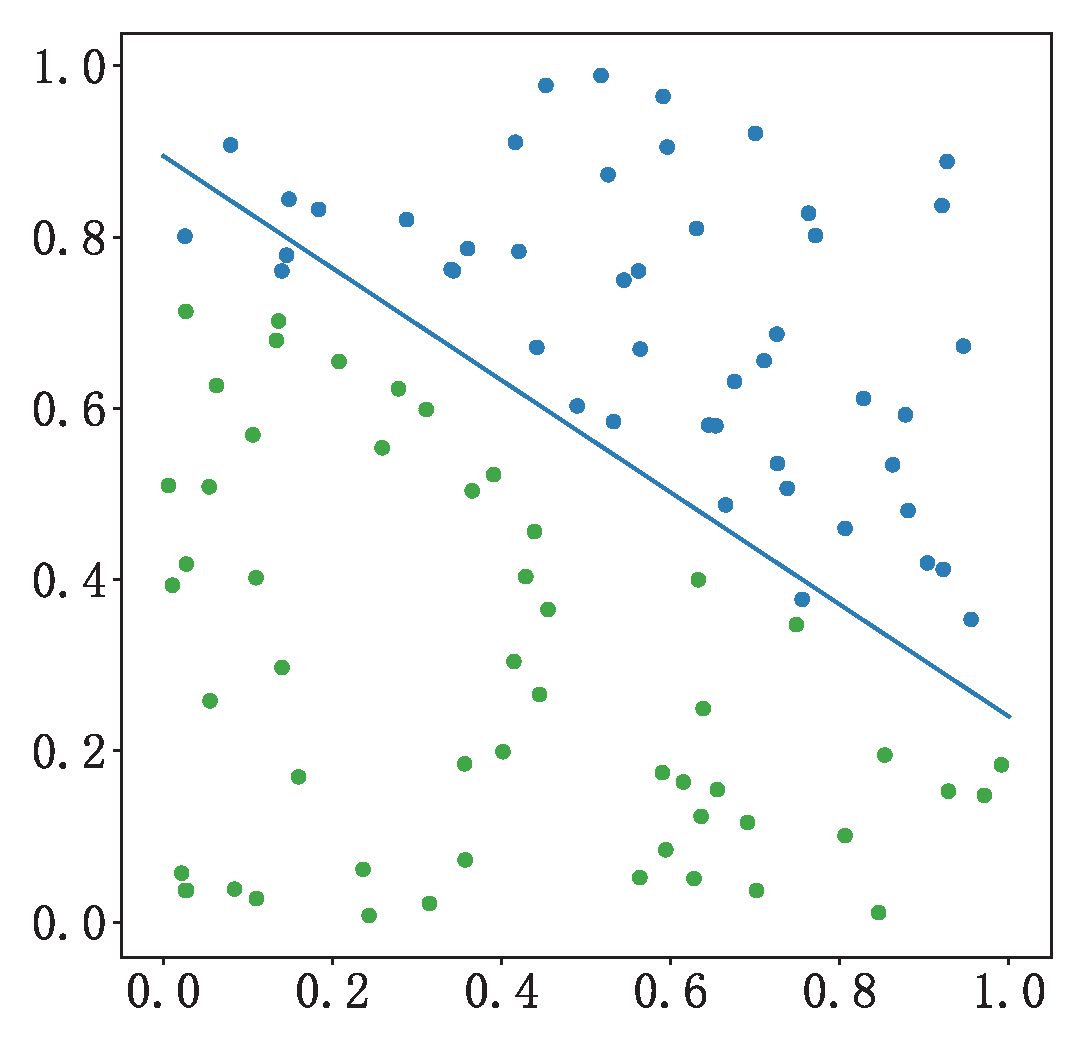
\includegraphics[scale=0.35]{500.eps}
            \end{minipage}
        }
        \subfigure[迭代2000次]
        {
            \begin{minipage}[b]{.45\linewidth}
                \centering
                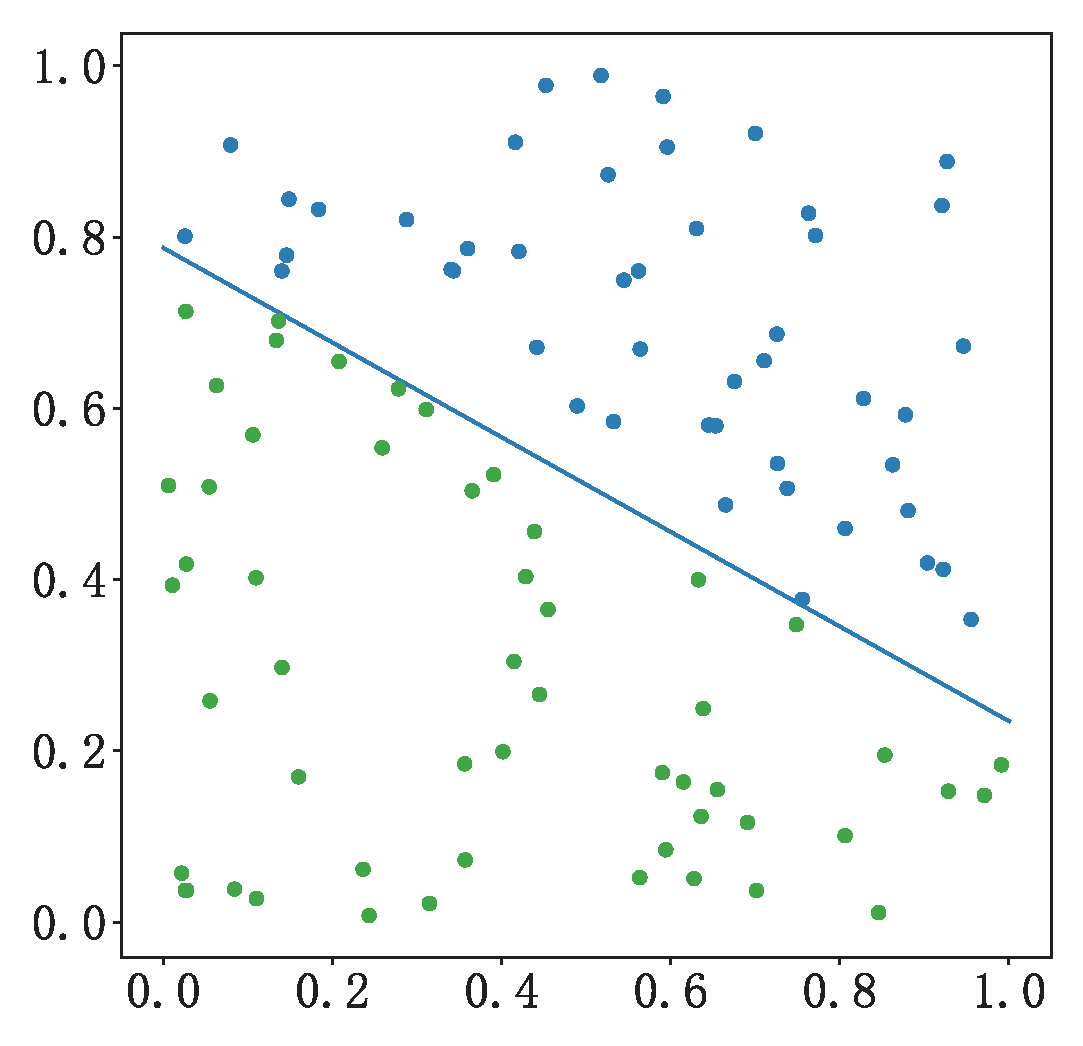
\includegraphics[scale=0.35]{2000.eps}
            \end{minipage}
        }
        \caption{迭代过程图}
        \label{figure-迭代过程图}
    \end{figure}
\fi
